\pagestyle{ima}
\label{ima}

%\begin{textblock*}{5.625in}(0pt,0pt)%
%\vspace*{-3.5cm}
%\hspace*{-2.77cm}\includegraphics*[width=175.2mm]{./propagandas/IMA.pdf}
%\end{textblock*}

%\pagebreak

\begin{center}
\hspace*{.5cm}\includegraphics[width=74mm]{./grid/bly.jpg}
\end{center}

\hspace*{-7cm}\hrulefill\hspace*{-7cm}

\medskip

\noindent{}Aos 21 anos, principiando no jornalismo, Nellie Bly partiu para Nova York à procura de emprego, onde foi desafiada por Joseph Pulitzer a investigar, pelo lado de dentro, um asilo mental acusado de maus"-tratos às pacientes. Fê"-lo com coragem e afinco. Hospedou"-se em uma pensão, onde fingiu ter um surto, foi detida pela polícia e examinada por um juiz e por médicos. Enganou a todos, foi tachada como louca irremediável e levada ao infame “Asilo de Loucos” da Ilha Blackwell, com a esperança de ser retirada de lá ao fim de dez dias. Dentro das grades do manicômio Nellie sofreu na pele, literalmente, os abusos de enfermeiras sádicas e o descaso de médicos incompetentes ou desinteressados. \hlc{O que mais a chocou, no entanto, foi encontrar entre as pacientes mulheres inteiramente sãs, tais como ela, mas pobres, doentes, imigrantes} que não falavam inglês ou ainda mulheres “indesejadas” por maridos, patrões ou familiares, convenientemente internadas e esquecidas.
O relato de seus dias no manicômio causou indignação nos leitores, o que levou a uma investigação pública e à demissão de médicos e enfermeiras.

%. Enfermeiras e médicos complacentes foram demitidos e a cidade investiu para que as pacientes tivessem uma vida minimamente digna. Foi a primeira matéria de Nellie que levou a um avanço concreto nos direitos humanos, e a ela seguiram-se outras reportagens transformadoras, incluindo denúncias de corrupção, tráfico de bebês e exploração de mulheres. Mais que uma desbravadora, Nellie Bly ajudou a fazer o mundo um pouco melhor, uma reportagem de cada vez.

\vfill

\hspace*{-.4cm}\begin{minipage}[c]{.5\linewidth}
\small\textbf{
\hspace*{-.1cm}Editora: Ímã Editorial\\
Título: Dez dias no manicômio\\
Autor: Nellie Bly\\ 
ISBN: 978-65-86419-05-4\\
Páginas: 206\\
Formato: 13x18cm\\
Preço: R\$ 42,00\\
}
\end{minipage}

\pagebreak

\vspace*{1.5cm}

\noindent{}{\nohyphens{\LARGE{Os dias de Nellie Bly no manicômio}}}

\bigskip

\hfill{}\scalebox{.8}{DANIELA ARBEX}

\bigskip
\bigskip
\bigskip

\begin{multicols}{2}
{\small\fakereceipt{
\noindent{}“Que lugar é este, perguntei ao homem
que tinha seus dedos afundados na carne
do meu braço. Ilha Blackwell — ele
respondeu — um lugar para loucos,
de onde você nunca mais vai sair.”
}}

\vspace{\baselineskip}

O diálogo acima foi travado em 1887 entre Nellie
Bly e um dos enfermeiros/carrascos que ela
encontrou no caminho para o “Asilo de Mulheres
Lunáticas”, o primeiro manicômio das Américas,
inaugurado quase 50 anos antes na cidade de
Nova York.

Aos 23 anos, a jornalista americana escreveu
seu nome na história (ou melhor, seu pseudônimo,
visto que se chamava de fato Elizabeth
Cochrane Seaman) após sentir na pele as violações
de direitos impostas a pessoas consideradas
em sofrimento psíquico. Para viver a experiência,
Bly se fez passar por louca, revelando as vulnerabilidades
de um sistema de atendimento que foi criado
justamente para alimentar o estigma da doença mental.

Apesar de plenamente sã, ela conseguiu
convencer médicos experientes e até um juiz a
decretarem"-na louca. Ao invés de procurarem
alguma pista sobre seu passado, os “donos da
razão” não hesitaram em despachá"-la para a ilha.
Nem mesmo a dúvida que pairava sobre sua
real enfermidade foi suficiente para garantir um
destino diferente ao da exclusão. Não demorou
muito para a então “paciente” descobrir que o
local confiscava a dignidade humana das mulheres
a quem se propunha cuidar.

No manicômio, a jovem repórter do \textit{The World},
jornal dirigido pelo famoso editor Joseph Pulitzer,
entendeu que o asilo tinha uma única finalidade:
manter entre seus muros todas as indesejáveis
sociais. Loucas ou não — muitas pacientes eram
apenas imigrantes que não dominavam o inglês
—, elas encontravam no asilo um lugar de silenciamento.
A instituição, na verdade, existia para
proteger os chamados “normais” daqueles que,
por convenção, foram transformados em escória.

O impressionante relato dos dez piores dias
da vida de Bly — que incluíram castigos físicos
e violência psicológica — vai além de um testemunho
pessoal. A potência dessa obra está
justamente na atualidade da sua denúncia.
A reportagem expõe uma lógica manicomial cruel que
segue fazendo milhões de vítimas ao redor do
mundo.

Ao escrever sobre a loucura, Bly fala em nome
de todas as pessoas que tiveram o direito básico
ao cuidado em liberdade negligenciado. O fato é
que aprisionar e excluir os diferentes revela muito
mais sobre uma cultura que ainda dialoga com o
higienismo do que propriamente sobre os considerados insanos.

Pioneira do jornalismo investigativo, a repórter
que manteve seu pseudônimo ao longo da
carreira conseguiu lançar luz sobre a
invisibilidade imposta aos loucos e às próprias mulheres.
Apesar de dois séculos terem se passado desde a
publicação do trabalho de Bly, a reportagem dela
continua colocando em xeque práticas que até
hoje não se propõem a tratar, mas a punir.

Feminista, Bly também teve um papel fundamental na conquista de direitos civis das americanas, como o direito ao voto em 1920. Suas
ideias, muito a frente do seu tempo, iluminaram
o caminho para que chegássemos até aqui. Bly
não é apenas sinônimo de coragem. Sua trajetória extraordinária é fonte de inspiração dos que seguem lutando na construção de uma sociedade
mais justa, solidária e humana.

\noindent{}\textcolor{gray}{\footnotesize\slsc{Adaptado do prefácio da edição de “Dez dias no manicômio”.}}
\end{multicols}


\pagebreak
\pagestyle{imacat}

\begin{multicols}{2}
\begin{enumerate}
\raggedright\nohyphens{
\item Marcelino, \textbf{Godofredo De Oliveira Neto}
\item Desamores da portuguesa, \textbf{Marta Barbosa Stephens}
\item Clube da esquina - Milton Nascimento e Lô Borges, \textbf{Milton Nascimento; Lô Borges; Charles Gavin}
\item Parasito, \textbf{Andrea Rangel}
\item Academia de danças - Egberto Gismonti, \textbf{Egberto Gismonti; Charles Gavin}
\item Secos \& Molhados, \textbf{Ney Matogrosso; Gerson Conrad; Charles Gavin}
\item 100 dias em Paris, \textbf{Tania Carvalho}
\item Perdidas, \textbf{Andrea del Fuego; Edney Silvestre; Henrique Rodrigues; Marcelo Moutinho; Marta Barbosa Stephens; Martha Batalha; Kátia Bandeira de Mello  Gerlach; Alexandre Staut} 
\item Rosa de ouro - Aracy Côrtes e Clementina de Jesus, \textbf{Hemínio Bello de Carvalho; Paulinho da Viola; Elton Medeiros; Charles Gavin}
\item Chico Buarque para todos, \textbf{Regina Zappa}
\item Galos de briga - João Bosco, \textbf{João Bosco; Charles Gavin}
\item Quem é quem - João Donato, \textbf{João Donato; Marcos Valle; Charles Gavin}
\item Dois - Legião Urbana, \textbf{Dado Villa-Lobos; Marcelo Bonfá; Charles Gavin}
\item Mulheres que mordem, \textbf{Beatriz Leal}
\item Nervos de aço - Paulinho da Viola, \textbf{Paulinho da Viola; Charles Gavin; Monarco}
\item Sociedade dividida, \textbf{Raphael Lima}
\item Estudando o samba - Tom Zé, \textbf{Tom Zé; Charles Gavin}
\item Reprograme, \textbf{Cory Doctorow; Nina Simon; Jane Finnis; Luis Marcelo Mendes}
\item Como o Botafogo conquistou a China, \textbf{Bruno Porto}
\item A peleja do diabo com o dono do céu -- Zé Ramalho, \textbf{Zé Ramalho; Charles Gavin}
\item A árvore oca, \textbf{Mauricio Vieira}
\item A morte visita Lisboa, \textbf{Fernando Perdigão}
\item Biografia do Língua, \textbf{Mario Lucio Sousa}
\item 100 dias em Lisboa, \textbf{Tania Carvalho}
\item A vagabunda, \textbf{Sidonie Gabrielle Colette}
}
\end{enumerate}
\end{multicols}

\pagebreak

%\hspace{.5cm}
%
%\begin{center}
%\hspace*{-.5cm}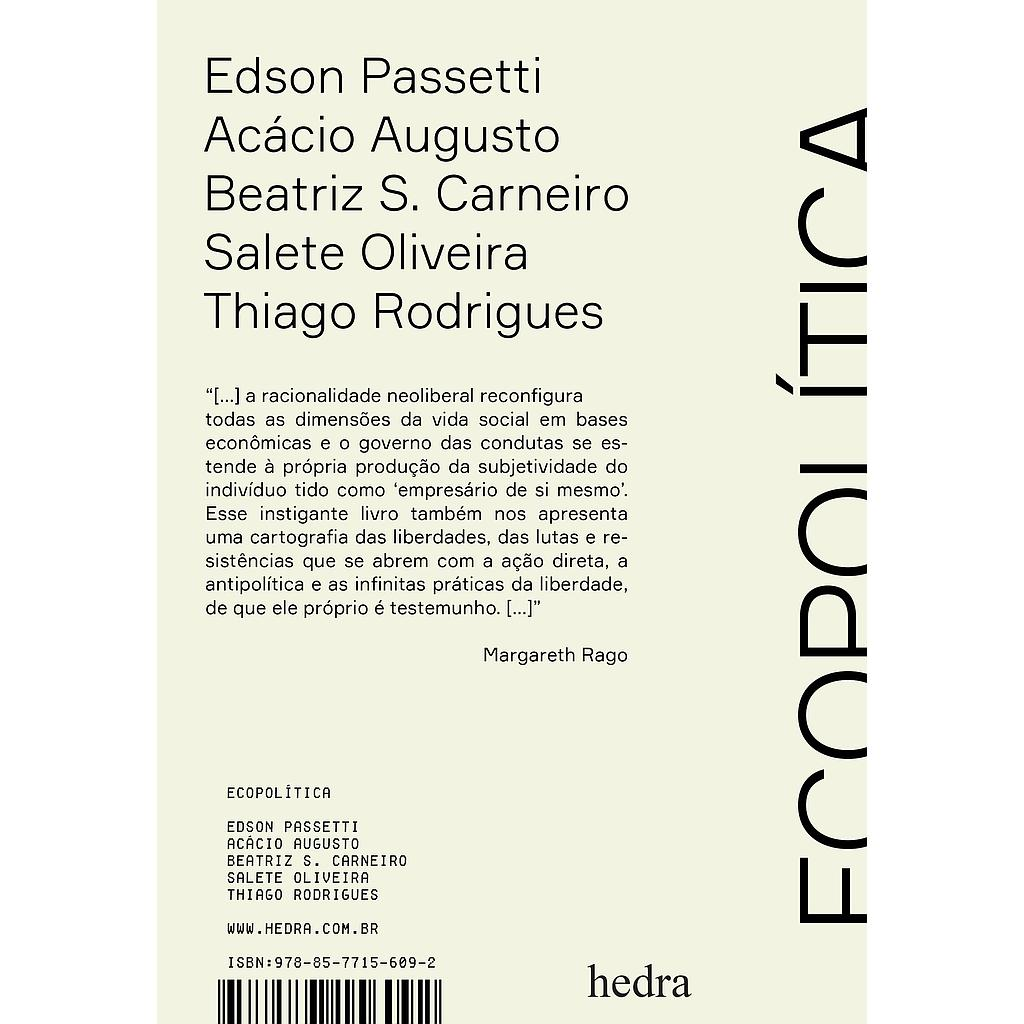
\includegraphics[width=70mm]{eco.jpeg}
%%\hspace*{6cm}\raisebox{2cm}{\rotatebox[origin=t]{90}\textbf{Lançamento}}}}
%\end{center}
%
%\hspace*{-2cm}\_\_\_\_\_\_\_\_\_\_\_\_\_\_\_\_\_\_\_\_\_\_\_\_\_\_\_\_\_\_\_\_\_\_\_\_\_\_\%_\_\_\_\_\_\_\_\_\_\_\_\_\_\_\_\_\_\_\_\_\_\_\_\_\_\_\_\_\_\_\_\_\_\_\_
%
%\medskip
%
%\noindent{}Lorem ipsum dolor sit amet, consectetur adipiscing elit.
%Donec sodales tortor a purus accumsan, ut ultricies purus
%maximus. Aliquam bibendum consequat mi, sed commo-
%do velit pellentesque id. Vivamus ultricies ligula in semper
%sagittis. Donec mollis odio in lectus tristique, sed convallis
%est interdum. Cras eget sem condimentum, pretium purus
%eu, auctor.
%
%\hspace{.5cm}
%
%\hspace*{-.4cm}\begin{minipage}[c]{0.45\linewidth}
%\small{
%\textbf{
%\hspace*{-.1cm}Título: Ecopolítica\\
%Autor: Edson Passetti\\ 
%Editora: Hedra\\
%Páginas: 476\\
%Formato: 23x16cm\\
%Preço: R\$ 79,90\\
%}}}}
%\end{minipage}
%\begin{minipage}[c]{0.50\linewidth}
%\small{Lorem ipsum dolor sit amet, consectetur adipiscing elit. onec sodales tortor a purus accumsan, ut ultricies. Lorem ipsum dolor sit amet, %consectetur adipiscing elit. Lorem ipsum dolor sit amet. Lorem ipsum dolor sit amet.} 
%\end{minipage}